\chapter{Introduction}
\label{ch:introduction}

\section{Preface}
\label{sec:preface}

Imagine being the owner of a piece of technology. It can be any physical device. Without maintenance, it is unavoidable that, after a certain amount of time of usage, it will have some sort of malfunction.
To overcome this problem, usually maintenance work is planned and performed by a team of skilled technicians. 

The simplest way of executing maintenance is to fix the device when it breaks. This is called \emph{reactive maintenance} (\gls{rm}). This has been done since forever, and it is still a very popular approach today, but it has a lot of drawbacks, ranging from the high downtime for repair, and the logistics of the spare parts etc.

The other family of maintenance techniques is called \emph{proactive maintenance} (\gls{pm}). All those techniques share the property of being applied before the device shows a malfunction. This is a very broad category, and it includes a lot of different techniques, most of which will be described in this thesis.

Back to the example, the owner of the device may want to avoid fixing it when it has already failed as much as possible, so the first improvement could be to perform maintenance periodically (on a schedule). This is called \emph{preventive maintenance} (\gls{pvm}). It's basically the same approach that every car owner uses to minimize the risk of the vehicle breaking down in the middle of the road. 
The owner may want to take the technique a step further and seek some sort of guidance on deciding when to perform maintenance. A very intuitive approach is to simply ask the skilled technicians to inspect all the devices very often to try to understand if something is wrong without interfering with the normal operation of the device.

If a technician has enough experience, he may be able to detect the vast majority of the problems before they become critical. He may do that simply using his senses, for example by listening to the sound of the device, or by touching it to feel how much it vibrates, how hot is it and so on. 

I would like to share, as a real-life example, what I witnessed during the commissioning of a new power plant. I remember that the commissioning manager (that is a chemist) was able to detect if the demineralization unit was working properly or not by simply tasting the water it produced, before the necessary instruments were installed.

This naive approach can be enhanced by using a large number of sensors to monitor the most critical parameters of the device. In this case, the technician will train himself more on the data of the sensors, rather than on inspecting the device directly. 

At this point, the next logical step would be to use the data from the sensor to train an algorithm, that will detect some patterns in the data that are not easily detectable by a human. This is called \emph{condition-based maintenance} (\gls{cbm}). This is the most common approach to \gls{pm} today. If this algorithm is trained only on the data taken when the device is working properly, it would only be able to detect a novel behavior, this is called \emph{novelty detection} (\gls{nd}). If the algorithm is trained on both the data taken when the device is working properly and the data taken when the device is malfunctioning in a specific way, it would be also able to detect the specific malfunction, this is called \emph{fault detection} (\gls{fd}).

One last improvement to the \gls{cbm} approach is to use an algorithm that will also try to predict how much time is left before a critical malfunction will occur. This approach is referred to as \emph{predictive maintenance} (\gls{pdm}). This is the most advanced approach to \gls{pm} today.

Both \gls{cbm} and \gls{pdm} could be done by using a model of the system that will predict the future behavior based on the current state of the system. The problem with this approach is that it is very difficult to build a model that is accurate enough to be useful. Most of the time, in industrial application, such a model is not available.
A workaround to this problem is to apply an Unsupervised Machine Learning (\gls{uml}) algorithm to the sensors data. This has the advantage of not needing a model of the system, but it has the drawback of being a black-box approach, so the parameters of the algorithm are not easily interpretable in a phisical sense. Furthermore, the algorithm will be fairly good at detecting anomalies, but it will have some limitations in predicting the future behavior of the system, since it will likely be based on a forecast done interpolating the data of the past.

\paragraph*{}
To visualize this evolution of maintenance approaches, let's have a look to \autoref{fig:earlysteamengine}. This is a purely mechanical device, so the only way to detect a malfunction before it causes a failure is by trusting the \quoted{gut feeling} of the operator. Moving on, the device in \autoref{fig:modernsteamengine} is also a steam engine, but it is equipped with some analogue gauges. In this case is it possible to define some thresholds for the readings that are indicative of a malfunction and look at the time evolution of the values. The measure of the sensor is immediatly displayed to the operator. Moving into present days, the device in \autoref{fig:controlroom} is a state of the art control room. The data from the sensors are elaborated by a computer and displayed to the operator on screens. This allows the computer to run algorithms on the sensor data.

\begin{figure}[htbp]
    \centering
    \begin{subfigure}{0.3\textwidth}  % <----
        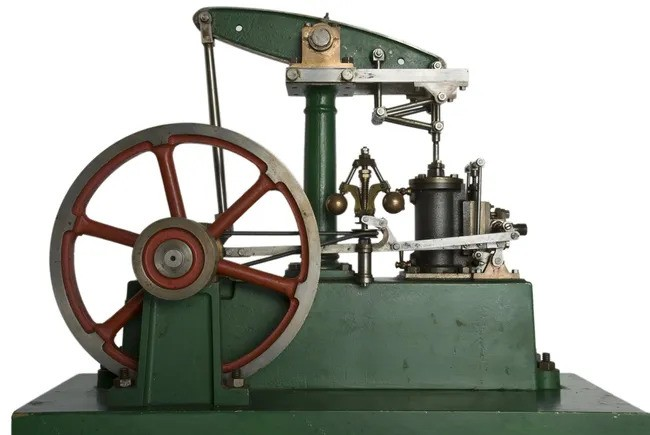
\includegraphics[width=\textwidth]{images/Intro/earlysteamengine.jpg}
        \caption{early steam engine \cite{steam_engine}}
        \label{fig:earlysteamengine}
    \end{subfigure}
    \begin{subfigure}{0.3\textwidth}  % <----
        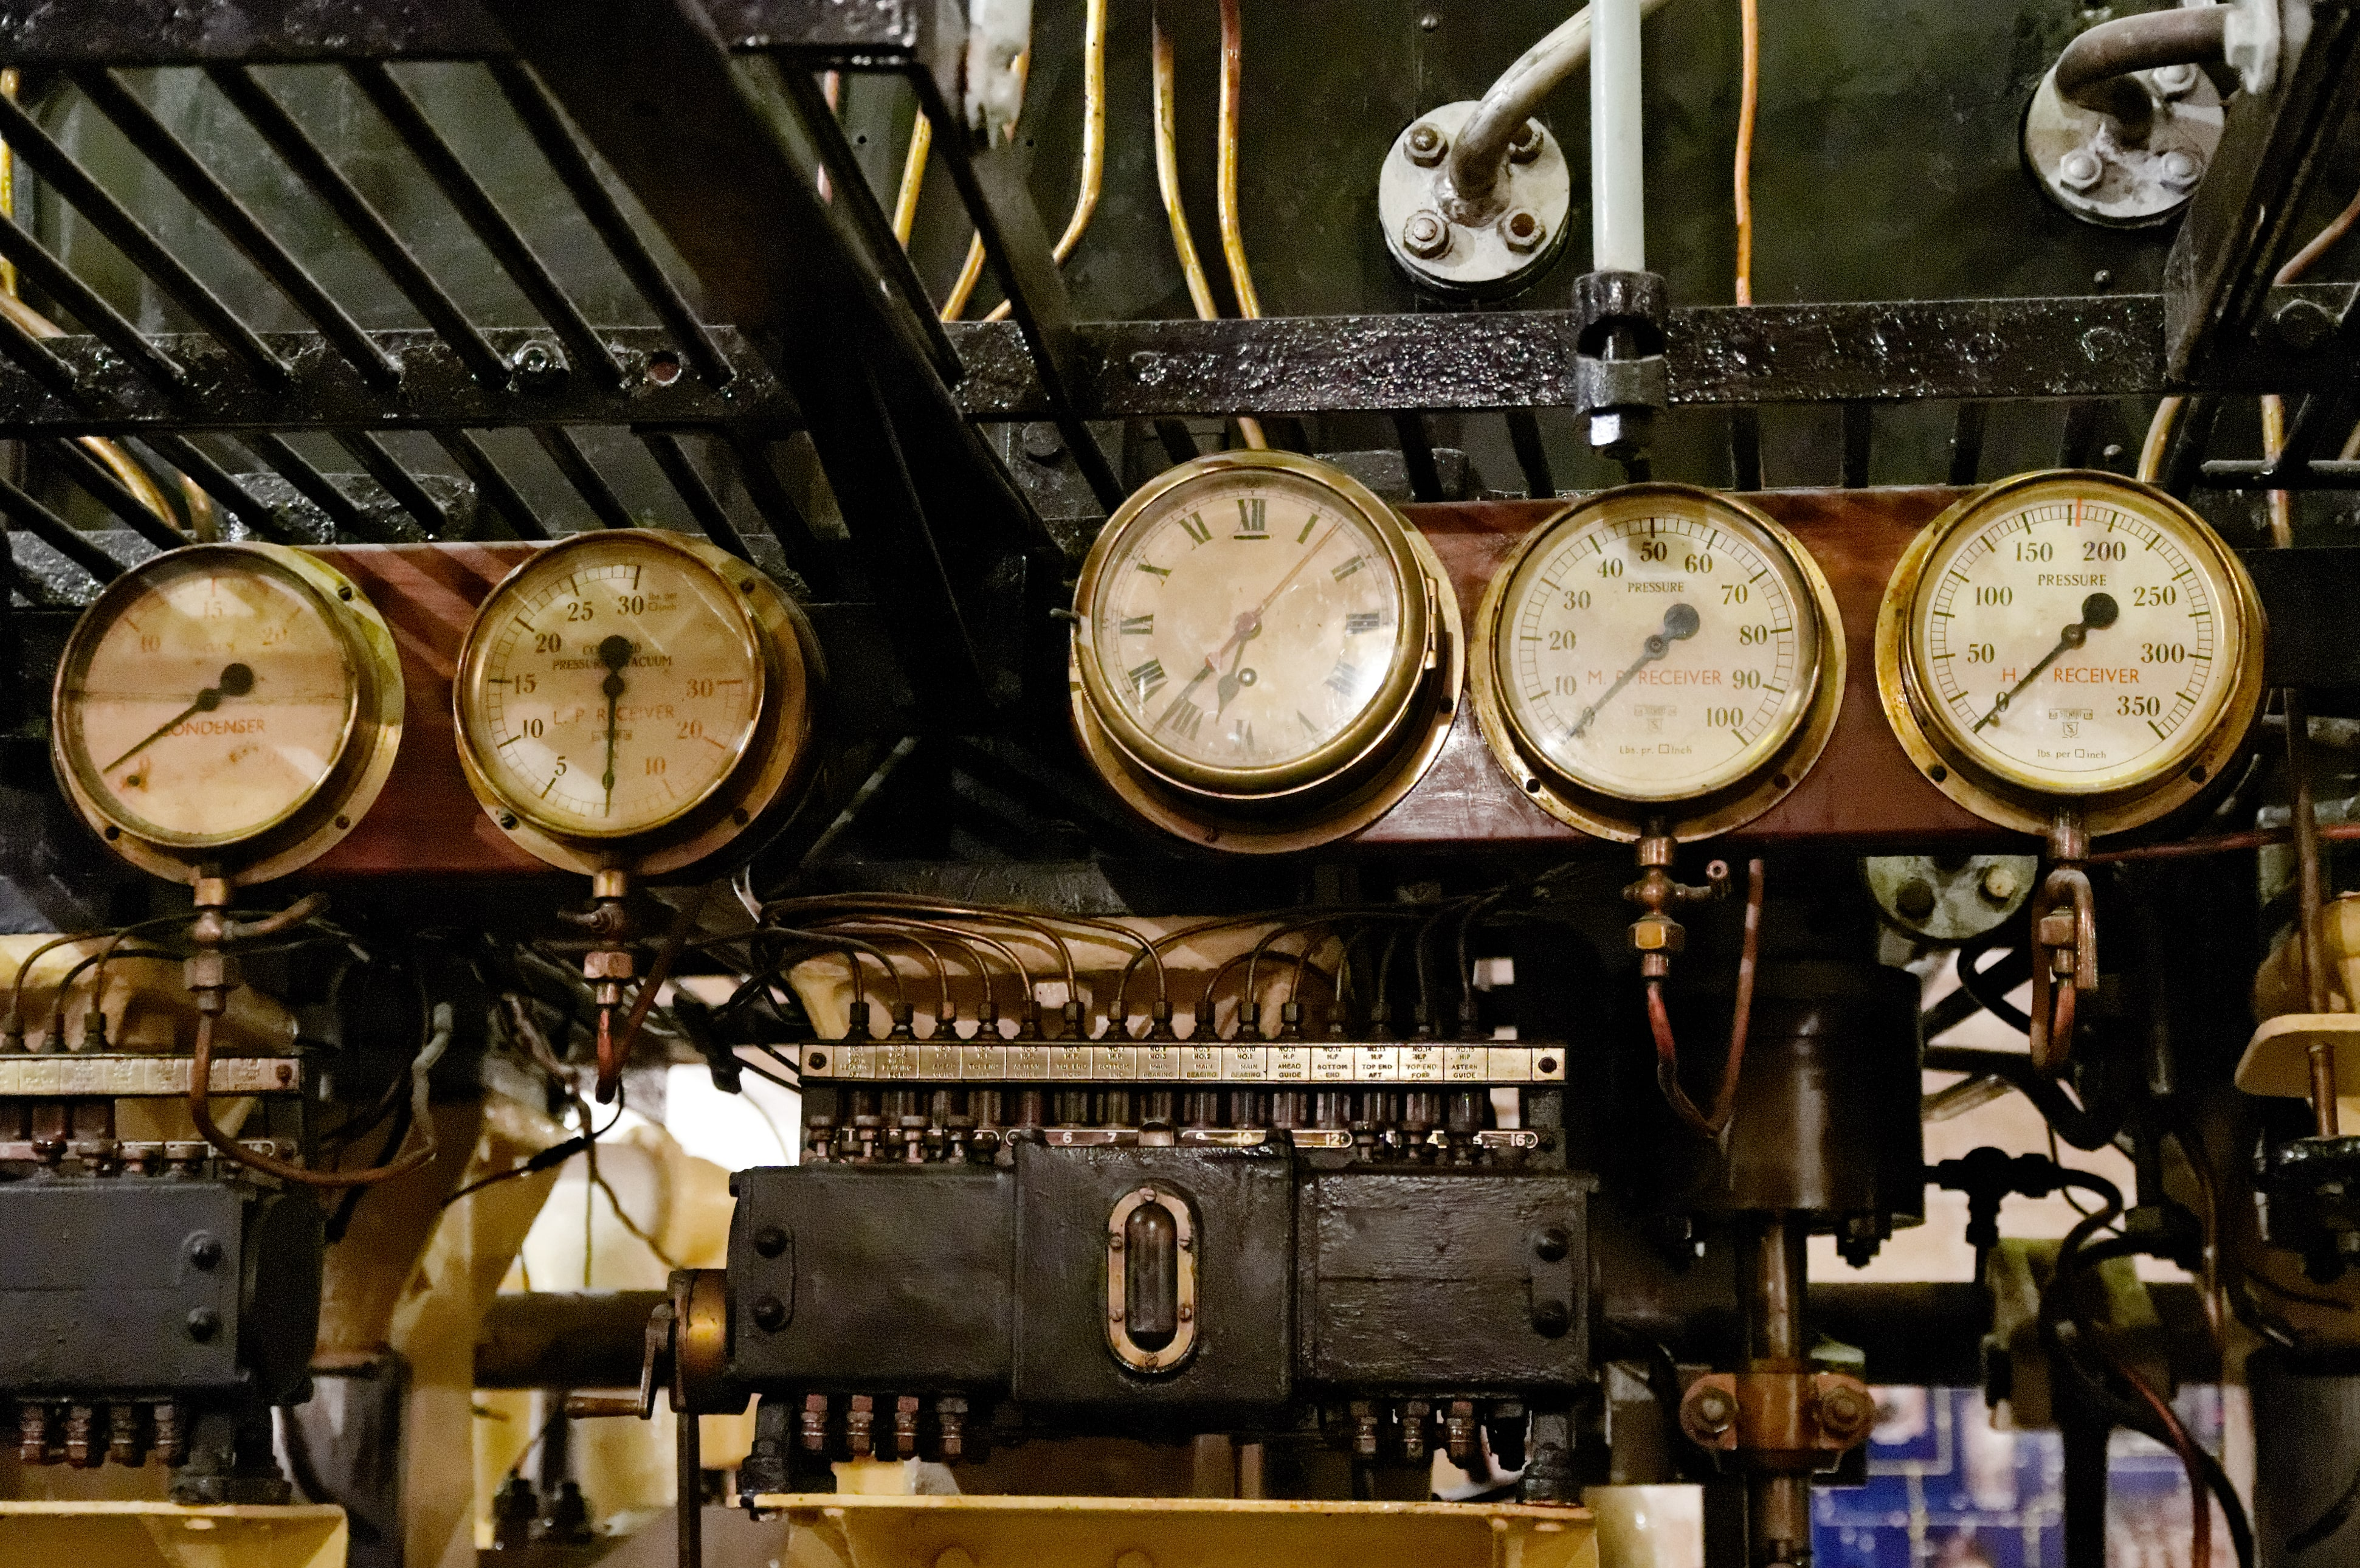
\includegraphics[width=\textwidth]{images/Intro/modernsteamengine.jpg}
        \caption{steam engine \cite{triple_expansion_engine}}
        \label{fig:modernsteamengine}
    \end{subfigure}
    \begin{subfigure}{0.3\textwidth}  % <----
        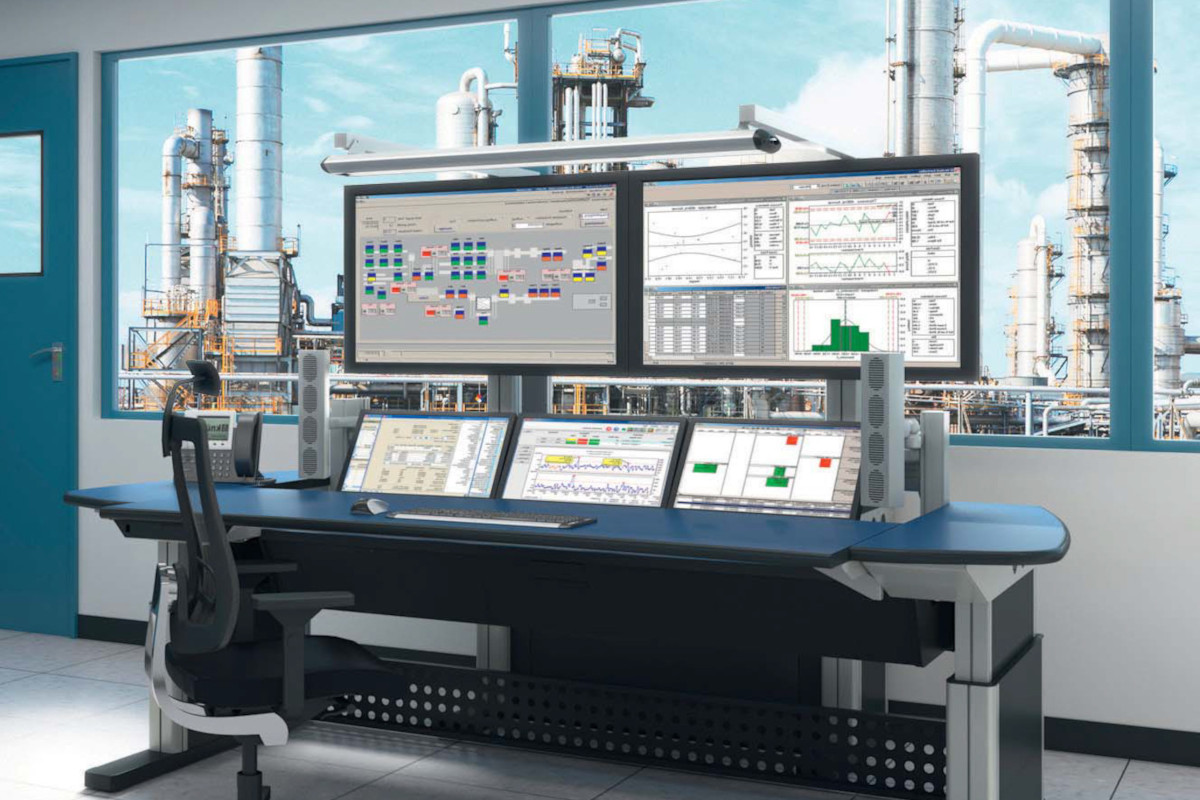
\includegraphics[width=\textwidth]{images/Intro/control-rooms-workstations.jpg}
        \caption{control room \cite{evosite}}
        \label{fig:controlroom}
    \end{subfigure}
    \caption{Evolution of machinery}
    \label{fig:machineryevolution}
\end{figure}

\paragraph*{}
The last comment is about where to run the algorithm. The most common approach is to run it un a server, that is not part of the device itself. This has the adventage of not having constraint on how much computational power is needed, because it's usually feasible to add more computational power to a computer that is not located on the device itself. The main drawback is that the data have to be transmitted to the server. This may not be feasible in some cases, for example for a mobile device, or for a device that is located in a remote area with no internet connection. In this case, the algorithm has to be run near the device itself, usually on a microcontroller that will perform an action when the algorithm detects a malfunction. This approach is called \emph{\gls{glo:edge}}. Using a microcontroller also has the advantage of using very little power, this is critical for battery-powered devices.



\section{Motivation}
\label{sec:motivation}

\begin{figure}
    \centering
    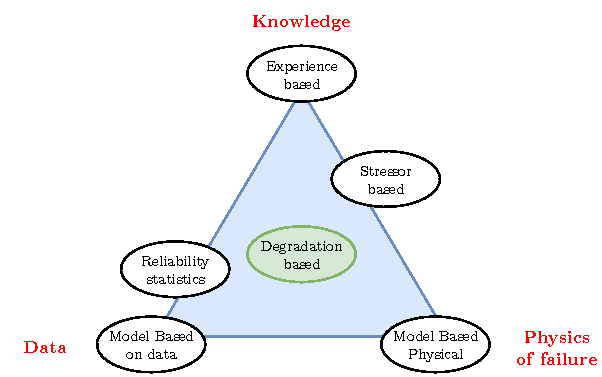
\includegraphics[scale=1.3]{images/Intro/MaintTriangle.pdf}
    \caption{Maintenance triangle}
    \label{fig:MaintTriangle}
\end{figure} 

Takin for example a survey published by the U.S. Department of Commerce in 2020, the maintenance expenditure of the manufacturing industry in the USA was \$57.3 billion, while the losses due to preventable maintenance issues amounted to \$119.1 billion. The top 25\% of those 
establishments relying on reactive maintenance were associated with 3.3 times more downtime 
than those in the bottom 25\% \cite{NIST}. This means that the economic impact of failures exceeds the cost of maintenance by a factor of 2.1, and this is concentrated in those sectors that rely more on reactive maintenance. The aforementioned emphasizes the importance of developing a general purpose \gls{pdm} system that can be applied in a large variety of systems.

In the article \cite{Maintenance_cat}, the authors divide the \gls{cbm} strategies in five categories:

\begin{itemize}
    \item \emph{experience based} predictions are based on the experience and knowledge outside or within the company. It is based on little scattered data on average conditions. The only  requirement is that the experience of the experts is quantified and used;
    \item \emph{reliability statistics} predictions are based on the statistical analysis of the failure data without considering the specific system. These methods also estimate the life
    of an average component operating under historically average conditions;
    \item \emph{stressor based} predictions can be considered an extension of the reliability statistics methods. The difference is that they also consider a measure of the stress (humidity, temperature, etc.) that the component is exposed to;
    \item \emph{degradation based} predictions are based on the extrapolation of the degradation of the component;
    \item \emph{model based} predictions are based on the knowledge of the physics of the system. The assumption is that the degradation can be computed instead of measured. They can be based on a physical model or on a data-driven model.
\end{itemize}


The authors of \cite{Maintenance_cat} also propose a distribution of these categories in a triangle, as shown in \autoref{fig:MaintTriangle}. Each vertex represents a requisite for the implementation, and the distance of the method to the vertex represents how dependent it is on that requisite. To obtain a general purpose \gls{pdm} framework, the \emph{degradation based} approach seems the most promising, since it is the least dependent on a specific requisite.

Moreover, to enhance even more the general purpose nature of the framework, a \gls{uml} model can be chosen. This speeds up the implementation of the framework on a machine about which little is known, plus, it can be implemented on a new machine without a deep knowledge of the \gls{uml} algorithms themself.

In the paper \cite{GridPredictMaintenance}, it is pointed out that \gls{glo:edge} implementations, not only enable the use of the framework for special applications but also enhance the cybersecurity of facilities that may not need an edge implementation due to technical limitations.
\section{Objective of the thesis}
\label{sec:objectives}

The goal of this thesis is to design, code and test a \gls{cbm} framework that will perform \gls{nd}, \gls{fd} and \gls{pdm}. This framework is thought to be general purpose, it needs just to receive time-series data from sensors, and set in training or evaluation mode.
This system will be implemented twice:
\begin{itemize}
    \item  coding in \texttt{python} and running it on a \gls{pc};
    \item   coding in \texttt{C} and running it on a microcontroller.
\end{itemize}

The development of the framework has been done modular and configurable, so that it can be easily adapted to different use cases. Things like the number of sensors, the sampling frequency, and the number and types of features to extract are easily configurable in a single file. The framework is also designed to be easily expandable, so that new features can be added simply by developing a method that appends the new feature to the feature vector, without the need to modify the rest of the framework.

To do that first a real bearing vibration dataset published by \cite{IMSpaper} has been analyzed to decide how to preprocess the data, which features to extract and which algorithm to use. 
The candidate algorithms described in \autoref{ch:Unsupervised} have been applied to the dataset and the results have been compared. These algorithms are \textbf{K-means}, \textbf{\gls{dbscan}}, \textbf{Gaussian Mixture Model}, \textbf{Isolation Forest}, \textbf{Local Outlier Factor} and \textbf{One-Class support vector machine}. 

All of the tests have been done trying to follow the most unsupervised approach possible, so the only information used to train the algorithm has been the data itself. Every user input needed by the algorithm has been chosen using an easily automatable method, to preserve the unsupervised nature of the framework that will be developed. For example, user inputs are the number of clusters in K-means, or the radius in the \gls{dbscan}.

At the end of the analysis, considering the trade-off between the performance of the algorithm, the computational cost and the simplicity, K-means has been chosen as the algorithm to implement in a real-time framework, developed in texttt{python}. Then, the data of the dataset was polled from a database at regular intervals and fed to the framework to simulate a real sensor polling the signal from the machine and evaluate the real-time performance of the implementation.

After that, a version of the framework with simplified architecture has been implemented in \texttt{C} and tested on a \texttt{STM32F767ZI} microcontroller board.

\section{Notations}
\label{sec:notations}
In this thesis, the following notations are used:
\begin{itemize}
  \item bold lowercase letters ($\vect{a}$, $\vect{b}$, $\vect{c}$) are used to denote vectors;
  \item italic lowercase letters ($a$, $b$, $c$) are used to denote scalars;
  \item bold uppercase letters ($\vect{A}$, $\vect{B}$, $\vect{C}$) are used to denote matrices;
  \item $\vect{a}_{i(j)}$ is the $j$th element of the vector $\vect{a}_i$;
  \item $||\vect{a}||_2$ is the $l^2$-norm of the vector $\vect{a}$, defined as $\sqrt{\sum_{i=1}^{n} a_i^2}$, denoted also as $\norm{a}$ for simplicity;
  \item $||\vect{a}||_n$ is the generic $l^n$-norm of the vector $\vect{a}$, defined as $\sqrt[n]{\sum_{i=1}^{n} \abs{a_i}^n}$;
  \item parenthesis encapsulating an index are used to condense descriptions, for example \quoted{\textbf{$\vect{a}_{i(j)}$ is the force applied to the $i$th ($j$th) step}} means that $\vect{a}_i$ is the force applied to the $i$th step and $\vect{a}_j$ is the force applied to the $j$th step;
  \item date and times are presented in the \gls{iso} 8601 format \cite{iso8601}. for example \texttt{YYYY-MM-DDThh:mm:ss}, where \texttt{T} is the date-time separator;
\end{itemize}

No distinction in notation is made between a vector in the phisycal sense (applied to a point, with a direction, and a magnitude) and a vector in the mathematical sense (a generic number $\in \mathbb{R}^n $).

As regard the flowcharts, the following symbols shown in \autoref{tab:flowsymbols} are used.


\begin{longtblr}[
  caption = {Symbols used in the flowcharts},
  label = {tab:flowsymbols},
]{
  cell{2}{1} = {t},
  cell{3}{1} = {t},
  cell{5}{1} = {t},
  cell{6}{1} = {t},
  cell{7}{1} = {t},
  hline{1,13} = {-}{0.08em},
  hline{2} = {-}{},
}
\textbf{Symbol} & \textbf{Name} & \textbf{Usage}\\
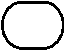
\includegraphics[scale=1]{images/FlowSymbols/terminator.pdf} & terminator & start or stop the process\\
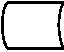
\includegraphics[scale=1]{images/FlowSymbols/storedData.pdf} & stored data & save some data\\
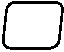
\includegraphics[scale=1]{images/FlowSymbols/data.pdf} & data & elaborate some data\\
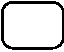
\includegraphics[scale=1]{images/FlowSymbols/process.pdf} & actions & perform automated actions\\
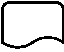
\includegraphics[scale=1]{images/FlowSymbols/document.pdf} & document & read or write a docuument\\
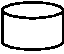
\includegraphics[scale=1]{images/FlowSymbols/database.pdf} & database & perform an action on a database\\
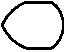
\includegraphics[scale=1]{images/FlowSymbols/display.pdf} & display & report, plot or display a value\\
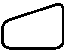
\includegraphics[scale=1]{images/FlowSymbols/manualInput.pdf} & manual input & request an input from the user\\
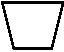
\includegraphics[scale=1]{images/FlowSymbols/manualOperation.pdf} & manual operation & request the user to do something\\
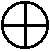
\includegraphics[scale=1]{images/FlowSymbols/or.pdf} & or & join flow line\\
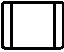
\includegraphics[scale=1]{images/FlowSymbols/predefProcess.pdf} & predefined process & run a programmed process
\end{longtblr}


%\printinunitsof{in}\prntlen{\textwidth}

% \begin{figure*}
%   \centering
% \begin{subfigure}{0.3\linewidth}  % <----
%  % This file was created with tikzplotlib v0.10.1.
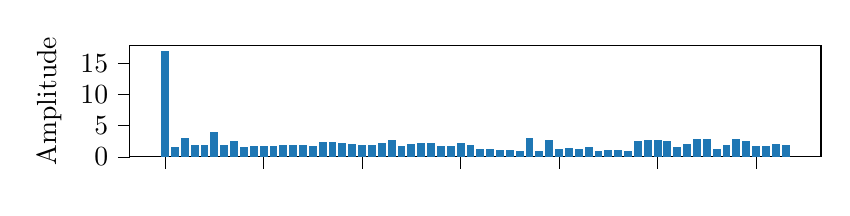
\begin{tikzpicture}

\definecolor{darkgray176}{RGB}{176,176,176}
\definecolor{steelblue31119180}{RGB}{31,119,180}

\begin{axis}[
height=3cm,
scaled x ticks=manual:{}{\pgfmathparse{#1}},
tick align=outside,
tick pos=left,
width=294.76926pt,
x grid style={darkgray176},
xmin=-3.59, xmax=66.59,
xtick style={color=black},
xticklabels={},
y grid style={darkgray176},
ylabel={Amplitude},
ymin=0, ymax=17.9224917606911,
ytick style={color=black},
ytick={0,5,10,15,20},
yticklabels={
  \(\displaystyle {0}\),
  \(\displaystyle {5}\),
  \(\displaystyle {10}\),
  \(\displaystyle {15}\),
  \(\displaystyle {20}\)
}
]
\draw[draw=none,fill=steelblue31119180] (axis cs:-0.4,0) rectangle (axis cs:0.4,17.0690397720867);
\draw[draw=none,fill=steelblue31119180] (axis cs:0.6,0) rectangle (axis cs:1.4,1.57701532870284);
\draw[draw=none,fill=steelblue31119180] (axis cs:1.6,0) rectangle (axis cs:2.4,3.04515592469192);
\draw[draw=none,fill=steelblue31119180] (axis cs:2.6,0) rectangle (axis cs:3.4,1.98727065046711);
\draw[draw=none,fill=steelblue31119180] (axis cs:3.6,0) rectangle (axis cs:4.4,1.87901229043815);
\draw[draw=none,fill=steelblue31119180] (axis cs:4.6,0) rectangle (axis cs:5.4,3.94494985947408);
\draw[draw=none,fill=steelblue31119180] (axis cs:5.6,0) rectangle (axis cs:6.4,1.94821362148988);
\draw[draw=none,fill=steelblue31119180] (axis cs:6.6,0) rectangle (axis cs:7.4,2.53456682074799);
\draw[draw=none,fill=steelblue31119180] (axis cs:7.6,0) rectangle (axis cs:8.4,1.53982779775888);
\draw[draw=none,fill=steelblue31119180] (axis cs:8.6,0) rectangle (axis cs:9.4,1.81855063876657);
\draw[draw=none,fill=steelblue31119180] (axis cs:9.6,0) rectangle (axis cs:10.4,1.74372106320514);
\draw[draw=none,fill=steelblue31119180] (axis cs:10.6,0) rectangle (axis cs:11.4,1.78981913351115);
\draw[draw=none,fill=steelblue31119180] (axis cs:11.6,0) rectangle (axis cs:12.4,1.9283565514217);
\draw[draw=none,fill=steelblue31119180] (axis cs:12.6,0) rectangle (axis cs:13.4,1.98727539890716);
\draw[draw=none,fill=steelblue31119180] (axis cs:13.6,0) rectangle (axis cs:14.4,1.83637697194901);
\draw[draw=none,fill=steelblue31119180] (axis cs:14.6,0) rectangle (axis cs:15.4,1.70629362470728);
\draw[draw=none,fill=steelblue31119180] (axis cs:15.6,0) rectangle (axis cs:16.4,2.32898911515285);
\draw[draw=none,fill=steelblue31119180] (axis cs:16.6,0) rectangle (axis cs:17.4,2.38726500121464);
\draw[draw=none,fill=steelblue31119180] (axis cs:17.6,0) rectangle (axis cs:18.4,2.2146470907513);
\draw[draw=none,fill=steelblue31119180] (axis cs:18.6,0) rectangle (axis cs:19.4,2.08886171015996);
\draw[draw=none,fill=steelblue31119180] (axis cs:19.6,0) rectangle (axis cs:20.4,1.91586717365543);
\draw[draw=none,fill=steelblue31119180] (axis cs:20.6,0) rectangle (axis cs:21.4,1.97741699428014);
\draw[draw=none,fill=steelblue31119180] (axis cs:21.6,0) rectangle (axis cs:22.4,2.26324345140917);
\draw[draw=none,fill=steelblue31119180] (axis cs:22.6,0) rectangle (axis cs:23.4,2.74150949309368);
\draw[draw=none,fill=steelblue31119180] (axis cs:23.6,0) rectangle (axis cs:24.4,1.67879784390802);
\draw[draw=none,fill=steelblue31119180] (axis cs:24.6,0) rectangle (axis cs:25.4,1.99560308046926);
\draw[draw=none,fill=steelblue31119180] (axis cs:25.6,0) rectangle (axis cs:26.4,2.18236194366914);
\draw[draw=none,fill=steelblue31119180] (axis cs:26.6,0) rectangle (axis cs:27.4,2.28116664486001);
\draw[draw=none,fill=steelblue31119180] (axis cs:27.6,0) rectangle (axis cs:28.4,1.76545125094874);
\draw[draw=none,fill=steelblue31119180] (axis cs:28.6,0) rectangle (axis cs:29.4,1.79936118428771);
\draw[draw=none,fill=steelblue31119180] (axis cs:29.6,0) rectangle (axis cs:30.4,2.21046386064049);
\draw[draw=none,fill=steelblue31119180] (axis cs:30.6,0) rectangle (axis cs:31.4,1.92512684988102);
\draw[draw=none,fill=steelblue31119180] (axis cs:31.6,0) rectangle (axis cs:32.4,1.29434219923151);
\draw[draw=none,fill=steelblue31119180] (axis cs:32.6,0) rectangle (axis cs:33.4,1.24905838096159);
\draw[draw=none,fill=steelblue31119180] (axis cs:33.6,0) rectangle (axis cs:34.4,1.0539404131426);
\draw[draw=none,fill=steelblue31119180] (axis cs:34.6,0) rectangle (axis cs:35.4,1.07785302549105);
\draw[draw=none,fill=steelblue31119180] (axis cs:35.6,0) rectangle (axis cs:36.4,1.00170991631713);
\draw[draw=none,fill=steelblue31119180] (axis cs:36.6,0) rectangle (axis cs:37.4,2.990570610034);
\draw[draw=none,fill=steelblue31119180] (axis cs:37.6,0) rectangle (axis cs:38.4,1.00976749017216);
\draw[draw=none,fill=steelblue31119180] (axis cs:38.6,0) rectangle (axis cs:39.4,2.77121989223762);
\draw[draw=none,fill=steelblue31119180] (axis cs:39.6,0) rectangle (axis cs:40.4,1.21267465980989);
\draw[draw=none,fill=steelblue31119180] (axis cs:40.6,0) rectangle (axis cs:41.4,1.44620941204964);
\draw[draw=none,fill=steelblue31119180] (axis cs:41.6,0) rectangle (axis cs:42.4,1.26138331095181);
\draw[draw=none,fill=steelblue31119180] (axis cs:42.6,0) rectangle (axis cs:43.4,1.60664374136418);
\draw[draw=none,fill=steelblue31119180] (axis cs:43.6,0) rectangle (axis cs:44.4,0.883196382772003);
\draw[draw=none,fill=steelblue31119180] (axis cs:44.6,0) rectangle (axis cs:45.4,1.0835546712407);
\draw[draw=none,fill=steelblue31119180] (axis cs:45.6,0) rectangle (axis cs:46.4,1.05267232084);
\draw[draw=none,fill=steelblue31119180] (axis cs:46.6,0) rectangle (axis cs:47.4,0.94061509525324);
\draw[draw=none,fill=steelblue31119180] (axis cs:47.6,0) rectangle (axis cs:48.4,2.5937245360833);
\draw[draw=none,fill=steelblue31119180] (axis cs:48.6,0) rectangle (axis cs:49.4,2.7964850933437);
\draw[draw=none,fill=steelblue31119180] (axis cs:49.6,0) rectangle (axis cs:50.4,2.71286149748853);
\draw[draw=none,fill=steelblue31119180] (axis cs:50.6,0) rectangle (axis cs:51.4,2.61834135486071);
\draw[draw=none,fill=steelblue31119180] (axis cs:51.6,0) rectangle (axis cs:52.4,1.64261763713365);
\draw[draw=none,fill=steelblue31119180] (axis cs:52.6,0) rectangle (axis cs:53.4,2.10765089952882);
\draw[draw=none,fill=steelblue31119180] (axis cs:53.6,0) rectangle (axis cs:54.4,2.79833649937833);
\draw[draw=none,fill=steelblue31119180] (axis cs:54.6,0) rectangle (axis cs:55.4,2.89223762573101);
\draw[draw=none,fill=steelblue31119180] (axis cs:55.6,0) rectangle (axis cs:56.4,1.32361974945306);
\draw[draw=none,fill=steelblue31119180] (axis cs:56.6,0) rectangle (axis cs:57.4,1.84030534558782);
\draw[draw=none,fill=steelblue31119180] (axis cs:57.6,0) rectangle (axis cs:58.4,2.82922380450697);
\draw[draw=none,fill=steelblue31119180] (axis cs:58.6,0) rectangle (axis cs:59.4,2.5822341294544);
\draw[draw=none,fill=steelblue31119180] (axis cs:59.6,0) rectangle (axis cs:60.4,1.71682916120663);
\draw[draw=none,fill=steelblue31119180] (axis cs:60.6,0) rectangle (axis cs:61.4,1.73398491114388);
\draw[draw=none,fill=steelblue31119180] (axis cs:61.6,0) rectangle (axis cs:62.4,2.13866133729592);
\draw[draw=none,fill=steelblue31119180] (axis cs:62.6,0) rectangle (axis cs:63.4,1.90570304888095);
\end{axis}

\end{tikzpicture}

%  \caption{Model 1}
%  \label{fig1a}
% \end{subfigure}

% \begin{subfigure}{0.3\linewidth}  % <----
%  % This file was created with tikzplotlib v0.10.1.
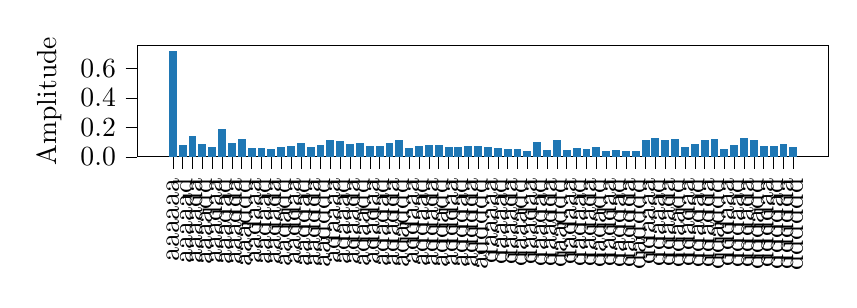
\begin{tikzpicture}

\definecolor{darkgray176}{RGB}{176,176,176}
\definecolor{steelblue31119180}{RGB}{31,119,180}

\begin{axis}[
height=3cm,
tick align=outside,
tick pos=left,
width=294.76926pt,
x grid style={darkgray176},
xmin=-3.59, xmax=66.59,
xtick style={color=black},
xtick={0,1,2,3,4,5,6,7,8,9,10,11,12,13,14,15,16,17,18,19,20,21,22,23,24,25,26,27,28,29,30,31,32,33,34,35,36,37,38,39,40,41,42,43,44,45,46,47,48,49,50,51,52,53,54,55,56,57,58,59,60,61,62,63},
xticklabel style={rotate=90.0},
xticklabels={
  aaaaaa,
  aaaaad,
  aaaada,
  aaaadd,
  aaadaa,
  aaadad,
  aaadda,
  aaaddd,
  aadaaa,
  aadaad,
  aadada,
  aadadd,
  aaddaa,
  aaddad,
  aaddda,
  aadddd,
  adaaaa,
  adaaad,
  adaada,
  adaadd,
  adadaa,
  adadad,
  adadda,
  adaddd,
  addaaa,
  addaad,
  addada,
  addadd,
  adddaa,
  adddad,
  adddda,
  addddd,
  daaaaa,
  daaaad,
  daaada,
  daaadd,
  daadaa,
  daadad,
  daadda,
  daaddd,
  dadaaa,
  dadaad,
  dadada,
  dadadd,
  daddaa,
  daddad,
  daddda,
  dadddd,
  ddaaaa,
  ddaaad,
  ddaada,
  ddaadd,
  ddadaa,
  ddadad,
  ddadda,
  ddaddd,
  dddaaa,
  dddaad,
  dddada,
  dddadd,
  ddddaa,
  ddddad,
  ddddda,
  dddddd
},
y grid style={darkgray176},
ylabel={Amplitude},
ymin=0, ymax=0.758179630791467,
ytick style={color=black},
ytick={0,0.2,0.4,0.6,0.8},
yticklabels={
  \(\displaystyle {0.0}\),
  \(\displaystyle {0.2}\),
  \(\displaystyle {0.4}\),
  \(\displaystyle {0.6}\),
  \(\displaystyle {0.8}\)
}
]
\draw[draw=none,fill=steelblue31119180] (axis cs:-0.4,0) rectangle (axis cs:0.4,0.722075838849016);
\draw[draw=none,fill=steelblue31119180] (axis cs:0.6,0) rectangle (axis cs:1.4,0.0816205118704516);
\draw[draw=none,fill=steelblue31119180] (axis cs:1.6,0) rectangle (axis cs:2.4,0.144788692125759);
\draw[draw=none,fill=steelblue31119180] (axis cs:2.6,0) rectangle (axis cs:3.4,0.0867045957893479);
\draw[draw=none,fill=steelblue31119180] (axis cs:3.6,0) rectangle (axis cs:4.4,0.0687644637243896);
\draw[draw=none,fill=steelblue31119180] (axis cs:4.6,0) rectangle (axis cs:5.4,0.191603550445973);
\draw[draw=none,fill=steelblue31119180] (axis cs:5.6,0) rectangle (axis cs:6.4,0.0912400814435433);
\draw[draw=none,fill=steelblue31119180] (axis cs:6.6,0) rectangle (axis cs:7.4,0.118441738979468);
\draw[draw=none,fill=steelblue31119180] (axis cs:7.6,0) rectangle (axis cs:8.4,0.063448949683056);
\draw[draw=none,fill=steelblue31119180] (axis cs:8.6,0) rectangle (axis cs:9.4,0.063549196660358);
\draw[draw=none,fill=steelblue31119180] (axis cs:9.6,0) rectangle (axis cs:10.4,0.0561566529115002);
\draw[draw=none,fill=steelblue31119180] (axis cs:10.6,0) rectangle (axis cs:11.4,0.0658459782078631);
\draw[draw=none,fill=steelblue31119180] (axis cs:11.6,0) rectangle (axis cs:12.4,0.0720379897131174);
\draw[draw=none,fill=steelblue31119180] (axis cs:12.6,0) rectangle (axis cs:13.4,0.0962993461770895);
\draw[draw=none,fill=steelblue31119180] (axis cs:13.6,0) rectangle (axis cs:14.4,0.0686195486369405);
\draw[draw=none,fill=steelblue31119180] (axis cs:14.6,0) rectangle (axis cs:15.4,0.0841955303823389);
\draw[draw=none,fill=steelblue31119180] (axis cs:15.6,0) rectangle (axis cs:16.4,0.114948175605847);
\draw[draw=none,fill=steelblue31119180] (axis cs:16.6,0) rectangle (axis cs:17.4,0.111103219250477);
\draw[draw=none,fill=steelblue31119180] (axis cs:17.6,0) rectangle (axis cs:18.4,0.0853474774953162);
\draw[draw=none,fill=steelblue31119180] (axis cs:18.6,0) rectangle (axis cs:19.4,0.0954229864952013);
\draw[draw=none,fill=steelblue31119180] (axis cs:19.6,0) rectangle (axis cs:20.4,0.0753330666191015);
\draw[draw=none,fill=steelblue31119180] (axis cs:20.6,0) rectangle (axis cs:21.4,0.0764573561609443);
\draw[draw=none,fill=steelblue31119180] (axis cs:21.6,0) rectangle (axis cs:22.4,0.0913486161286602);
\draw[draw=none,fill=steelblue31119180] (axis cs:22.6,0) rectangle (axis cs:23.4,0.115440781780618);
\draw[draw=none,fill=steelblue31119180] (axis cs:23.6,0) rectangle (axis cs:24.4,0.0605363919448476);
\draw[draw=none,fill=steelblue31119180] (axis cs:24.6,0) rectangle (axis cs:25.4,0.0715006546875076);
\draw[draw=none,fill=steelblue31119180] (axis cs:25.6,0) rectangle (axis cs:26.4,0.0834816059877538);
\draw[draw=none,fill=steelblue31119180] (axis cs:26.6,0) rectangle (axis cs:27.4,0.0825718187220844);
\draw[draw=none,fill=steelblue31119180] (axis cs:27.6,0) rectangle (axis cs:28.4,0.0657381299772261);
\draw[draw=none,fill=steelblue31119180] (axis cs:28.6,0) rectangle (axis cs:29.4,0.0684981211033183);
\draw[draw=none,fill=steelblue31119180] (axis cs:29.6,0) rectangle (axis cs:30.4,0.0735247581287173);
\draw[draw=none,fill=steelblue31119180] (axis cs:30.6,0) rectangle (axis cs:31.4,0.0714264975904106);
\draw[draw=none,fill=steelblue31119180] (axis cs:31.6,0) rectangle (axis cs:32.4,0.0674403501539547);
\draw[draw=none,fill=steelblue31119180] (axis cs:32.6,0) rectangle (axis cs:33.4,0.0592824747919798);
\draw[draw=none,fill=steelblue31119180] (axis cs:33.6,0) rectangle (axis cs:34.4,0.052030899559776);
\draw[draw=none,fill=steelblue31119180] (axis cs:34.6,0) rectangle (axis cs:35.4,0.0513258807665482);
\draw[draw=none,fill=steelblue31119180] (axis cs:35.6,0) rectangle (axis cs:36.4,0.0416017100177299);
\draw[draw=none,fill=steelblue31119180] (axis cs:36.6,0) rectangle (axis cs:37.4,0.101744455756126);
\draw[draw=none,fill=steelblue31119180] (axis cs:37.6,0) rectangle (axis cs:38.4,0.0463410493438625);
\draw[draw=none,fill=steelblue31119180] (axis cs:38.6,0) rectangle (axis cs:39.4,0.117328390407309);
\draw[draw=none,fill=steelblue31119180] (axis cs:39.6,0) rectangle (axis cs:40.4,0.0462494158731625);
\draw[draw=none,fill=steelblue31119180] (axis cs:40.6,0) rectangle (axis cs:41.4,0.0593257131667686);
\draw[draw=none,fill=steelblue31119180] (axis cs:41.6,0) rectangle (axis cs:42.4,0.0526934179057522);
\draw[draw=none,fill=steelblue31119180] (axis cs:42.6,0) rectangle (axis cs:43.4,0.0668781753176304);
\draw[draw=none,fill=steelblue31119180] (axis cs:43.6,0) rectangle (axis cs:44.4,0.0416416018534089);
\draw[draw=none,fill=steelblue31119180] (axis cs:44.6,0) rectangle (axis cs:45.4,0.0462760456257271);
\draw[draw=none,fill=steelblue31119180] (axis cs:45.6,0) rectangle (axis cs:46.4,0.0434239384103015);
\draw[draw=none,fill=steelblue31119180] (axis cs:46.6,0) rectangle (axis cs:47.4,0.0416410127228071);
\draw[draw=none,fill=steelblue31119180] (axis cs:47.6,0) rectangle (axis cs:48.4,0.117322919554115);
\draw[draw=none,fill=steelblue31119180] (axis cs:48.6,0) rectangle (axis cs:49.4,0.130187409367646);
\draw[draw=none,fill=steelblue31119180] (axis cs:49.6,0) rectangle (axis cs:50.4,0.114133627497582);
\draw[draw=none,fill=steelblue31119180] (axis cs:50.6,0) rectangle (axis cs:51.4,0.121358917513582);
\draw[draw=none,fill=steelblue31119180] (axis cs:51.6,0) rectangle (axis cs:52.4,0.0707478156876725);
\draw[draw=none,fill=steelblue31119180] (axis cs:52.6,0) rectangle (axis cs:53.4,0.0878711098289786);
\draw[draw=none,fill=steelblue31119180] (axis cs:53.6,0) rectangle (axis cs:54.4,0.112974228550204);
\draw[draw=none,fill=steelblue31119180] (axis cs:54.6,0) rectangle (axis cs:55.4,0.120443137445082);
\draw[draw=none,fill=steelblue31119180] (axis cs:55.6,0) rectangle (axis cs:56.4,0.053252675940857);
\draw[draw=none,fill=steelblue31119180] (axis cs:56.6,0) rectangle (axis cs:57.4,0.077975346334595);
\draw[draw=none,fill=steelblue31119180] (axis cs:57.6,0) rectangle (axis cs:58.4,0.125489421529731);
\draw[draw=none,fill=steelblue31119180] (axis cs:58.6,0) rectangle (axis cs:59.4,0.113761107750516);
\draw[draw=none,fill=steelblue31119180] (axis cs:59.6,0) rectangle (axis cs:60.4,0.0721800422035524);
\draw[draw=none,fill=steelblue31119180] (axis cs:60.6,0) rectangle (axis cs:61.4,0.0753054888730634);
\draw[draw=none,fill=steelblue31119180] (axis cs:61.6,0) rectangle (axis cs:62.4,0.0854419009187501);
\draw[draw=none,fill=steelblue31119180] (axis cs:62.6,0) rectangle (axis cs:63.4,0.0676569727174981);
\end{axis}

\end{tikzpicture}

%  \caption{Model 2}
%  \label{fig1b}
% \end{subfigure}

% \begin{subfigure}{0.3\linewidth}  % <----
%  % This file was created with tikzplotlib v0.10.1.
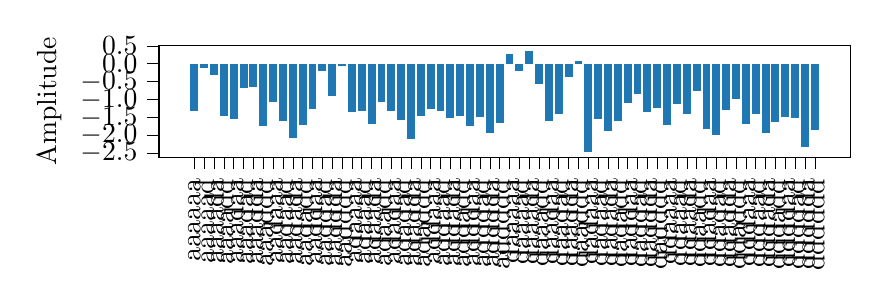
\begin{tikzpicture}

\definecolor{darkgray176}{RGB}{176,176,176}
\definecolor{steelblue31119180}{RGB}{31,119,180}

\begin{axis}[
height=3cm,
tick align=outside,
tick pos=left,
width=294.76926pt,
x grid style={darkgray176},
xmin=-3.59, xmax=66.59,
xtick style={color=black},
xtick={0,1,2,3,4,5,6,7,8,9,10,11,12,13,14,15,16,17,18,19,20,21,22,23,24,25,26,27,28,29,30,31,32,33,34,35,36,37,38,39,40,41,42,43,44,45,46,47,48,49,50,51,52,53,54,55,56,57,58,59,60,61,62,63},
xticklabel style={rotate=90.0},
xticklabels={
  aaaaaa,
  aaaaad,
  aaaada,
  aaaadd,
  aaadaa,
  aaadad,
  aaadda,
  aaaddd,
  aadaaa,
  aadaad,
  aadada,
  aadadd,
  aaddaa,
  aaddad,
  aaddda,
  aadddd,
  adaaaa,
  adaaad,
  adaada,
  adaadd,
  adadaa,
  adadad,
  adadda,
  adaddd,
  addaaa,
  addaad,
  addada,
  addadd,
  adddaa,
  adddad,
  adddda,
  addddd,
  daaaaa,
  daaaad,
  daaada,
  daaadd,
  daadaa,
  daadad,
  daadda,
  daaddd,
  dadaaa,
  dadaad,
  dadada,
  dadadd,
  daddaa,
  daddad,
  daddda,
  dadddd,
  ddaaaa,
  ddaaad,
  ddaada,
  ddaadd,
  ddadaa,
  ddadad,
  ddadda,
  ddaddd,
  dddaaa,
  dddaad,
  dddada,
  dddadd,
  ddddaa,
  ddddad,
  ddddda,
  dddddd
},
y grid style={darkgray176},
ylabel={Amplitude},
ymin=-2.61740256008719, ymax=0.509919465810349,
ytick style={color=black},
ytick={-3,-2.5,-2,-1.5,-1,-0.5,0,0.5,1},
yticklabels={
  \(\displaystyle {\ensuremath{-}3.0}\),
  \(\displaystyle {\ensuremath{-}2.5}\),
  \(\displaystyle {\ensuremath{-}2.0}\),
  \(\displaystyle {\ensuremath{-}1.5}\),
  \(\displaystyle {\ensuremath{-}1.0}\),
  \(\displaystyle {\ensuremath{-}0.5}\),
  \(\displaystyle {0.0}\),
  \(\displaystyle {0.5}\),
  \(\displaystyle {1.0}\)
}
]
\draw[draw=none,fill=steelblue31119180] (axis cs:-0.4,0) rectangle (axis cs:0.4,-1.31463451570886);
\draw[draw=none,fill=steelblue31119180] (axis cs:0.6,0) rectangle (axis cs:1.4,-0.134818691790791);
\draw[draw=none,fill=steelblue31119180] (axis cs:1.6,0) rectangle (axis cs:2.4,-0.319435036080992);
\draw[draw=none,fill=steelblue31119180] (axis cs:2.6,0) rectangle (axis cs:3.4,-1.45257985930736);
\draw[draw=none,fill=steelblue31119180] (axis cs:3.6,0) rectangle (axis cs:4.4,-1.5421469645371);
\draw[draw=none,fill=steelblue31119180] (axis cs:4.6,0) rectangle (axis cs:5.4,-0.673764853725896);
\draw[draw=none,fill=steelblue31119180] (axis cs:5.6,0) rectangle (axis cs:6.4,-0.651067231629759);
\draw[draw=none,fill=steelblue31119180] (axis cs:6.6,0) rectangle (axis cs:7.4,-1.74945636196658);
\draw[draw=none,fill=steelblue31119180] (axis cs:7.6,0) rectangle (axis cs:8.4,-1.07894447704247);
\draw[draw=none,fill=steelblue31119180] (axis cs:8.6,0) rectangle (axis cs:9.4,-1.611860529353);
\draw[draw=none,fill=steelblue31119180] (axis cs:9.6,0) rectangle (axis cs:10.4,-2.08587288612999);
\draw[draw=none,fill=steelblue31119180] (axis cs:10.6,0) rectangle (axis cs:11.4,-1.70951336361917);
\draw[draw=none,fill=steelblue31119180] (axis cs:11.6,0) rectangle (axis cs:12.4,-1.28157675228911);
\draw[draw=none,fill=steelblue31119180] (axis cs:12.6,0) rectangle (axis cs:13.4,-0.197861624149187);
\draw[draw=none,fill=steelblue31119180] (axis cs:13.6,0) rectangle (axis cs:14.4,-0.902246969989867);
\draw[draw=none,fill=steelblue31119180] (axis cs:14.6,0) rectangle (axis cs:15.4,-0.0599945188814577);
\draw[draw=none,fill=steelblue31119180] (axis cs:15.6,0) rectangle (axis cs:16.4,-1.36541350319367);
\draw[draw=none,fill=steelblue31119180] (axis cs:16.6,0) rectangle (axis cs:17.4,-1.3266188419031);
\draw[draw=none,fill=steelblue31119180] (axis cs:17.6,0) rectangle (axis cs:18.4,-1.69808295679741);
\draw[draw=none,fill=steelblue31119180] (axis cs:18.6,0) rectangle (axis cs:19.4,-1.08150865222734);
\draw[draw=none,fill=steelblue31119180] (axis cs:19.6,0) rectangle (axis cs:20.4,-1.3300365540605);
\draw[draw=none,fill=steelblue31119180] (axis cs:20.6,0) rectangle (axis cs:21.4,-1.56591194958796);
\draw[draw=none,fill=steelblue31119180] (axis cs:21.6,0) rectangle (axis cs:22.4,-2.10018255300044);
\draw[draw=none,fill=steelblue31119180] (axis cs:22.6,0) rectangle (axis cs:23.4,-1.46373211270423);
\draw[draw=none,fill=steelblue31119180] (axis cs:23.6,0) rectangle (axis cs:24.4,-1.27545670892696);
\draw[draw=none,fill=steelblue31119180] (axis cs:24.6,0) rectangle (axis cs:25.4,-1.33850245699865);
\draw[draw=none,fill=steelblue31119180] (axis cs:25.6,0) rectangle (axis cs:26.4,-1.52906230329855);
\draw[draw=none,fill=steelblue31119180] (axis cs:26.6,0) rectangle (axis cs:27.4,-1.45230662679311);
\draw[draw=none,fill=steelblue31119180] (axis cs:27.6,0) rectangle (axis cs:28.4,-1.73255965580102);
\draw[draw=none,fill=steelblue31119180] (axis cs:28.6,0) rectangle (axis cs:29.4,-1.50335007709024);
\draw[draw=none,fill=steelblue31119180] (axis cs:29.6,0) rectangle (axis cs:30.4,-1.94720337219532);
\draw[draw=none,fill=steelblue31119180] (axis cs:30.6,0) rectangle (axis cs:31.4,-1.65528675483821);
\draw[draw=none,fill=steelblue31119180] (axis cs:31.6,0) rectangle (axis cs:32.4,0.270054443767034);
\draw[draw=none,fill=steelblue31119180] (axis cs:32.6,0) rectangle (axis cs:33.4,-0.197751373312009);
\draw[draw=none,fill=steelblue31119180] (axis cs:33.6,0) rectangle (axis cs:34.4,0.367768464633188);
\draw[draw=none,fill=steelblue31119180] (axis cs:34.6,0) rectangle (axis cs:35.4,-0.564735648791296);
\draw[draw=none,fill=steelblue31119180] (axis cs:35.6,0) rectangle (axis cs:36.4,-1.61150252577791);
\draw[draw=none,fill=steelblue31119180] (axis cs:36.6,0) rectangle (axis cs:37.4,-1.40564010823609);
\draw[draw=none,fill=steelblue31119180] (axis cs:37.6,0) rectangle (axis cs:38.4,-0.371182760704031);
\draw[draw=none,fill=steelblue31119180] (axis cs:38.6,0) rectangle (axis cs:39.4,0.070349641149425);
\draw[draw=none,fill=steelblue31119180] (axis cs:39.6,0) rectangle (axis cs:40.4,-2.47525155891003);
\draw[draw=none,fill=steelblue31119180] (axis cs:40.6,0) rectangle (axis cs:41.4,-1.55614989351769);
\draw[draw=none,fill=steelblue31119180] (axis cs:41.6,0) rectangle (axis cs:42.4,-1.88234123808839);
\draw[draw=none,fill=steelblue31119180] (axis cs:42.6,0) rectangle (axis cs:43.4,-1.59270070771934);
\draw[draw=none,fill=steelblue31119180] (axis cs:43.6,0) rectangle (axis cs:44.4,-1.11190650381437);
\draw[draw=none,fill=steelblue31119180] (axis cs:44.6,0) rectangle (axis cs:45.4,-0.840681397994204);
\draw[draw=none,fill=steelblue31119180] (axis cs:45.6,0) rectangle (axis cs:46.4,-1.34368535787999);
\draw[draw=none,fill=steelblue31119180] (axis cs:46.6,0) rectangle (axis cs:47.4,-1.25517956985282);
\draw[draw=none,fill=steelblue31119180] (axis cs:47.6,0) rectangle (axis cs:48.4,-1.7101579930862);
\draw[draw=none,fill=steelblue31119180] (axis cs:48.6,0) rectangle (axis cs:49.4,-1.14244936083466);
\draw[draw=none,fill=steelblue31119180] (axis cs:49.6,0) rectangle (axis cs:50.4,-1.41050679464651);
\draw[draw=none,fill=steelblue31119180] (axis cs:50.6,0) rectangle (axis cs:51.4,-0.772205746905425);
\draw[draw=none,fill=steelblue31119180] (axis cs:51.6,0) rectangle (axis cs:52.4,-1.82325501180065);
\draw[draw=none,fill=steelblue31119180] (axis cs:52.6,0) rectangle (axis cs:53.4,-1.99315327974258);
\draw[draw=none,fill=steelblue31119180] (axis cs:53.6,0) rectangle (axis cs:54.4,-1.29641163379117);
\draw[draw=none,fill=steelblue31119180] (axis cs:54.6,0) rectangle (axis cs:55.4,-0.990550307115663);
\draw[draw=none,fill=steelblue31119180] (axis cs:55.6,0) rectangle (axis cs:56.4,-1.6980346169395);
\draw[draw=none,fill=steelblue31119180] (axis cs:56.6,0) rectangle (axis cs:57.4,-1.42284013393087);
\draw[draw=none,fill=steelblue31119180] (axis cs:57.6,0) rectangle (axis cs:58.4,-1.94315047574371);
\draw[draw=none,fill=steelblue31119180] (axis cs:58.6,0) rectangle (axis cs:59.4,-1.62789056222075);
\draw[draw=none,fill=steelblue31119180] (axis cs:59.6,0) rectangle (axis cs:60.4,-1.48520306606731);
\draw[draw=none,fill=steelblue31119180] (axis cs:60.6,0) rectangle (axis cs:61.4,-1.50855956912423);
\draw[draw=none,fill=steelblue31119180] (axis cs:61.6,0) rectangle (axis cs:62.4,-2.32843343387864);
\draw[draw=none,fill=steelblue31119180] (axis cs:62.6,0) rectangle (axis cs:63.4,-1.84413382243553);
\end{axis}

\end{tikzpicture}

%  \caption{Model 2}
%  \label{fig1b}
% \end{subfigure}

% \caption{Models}
% \label{fig2}
% \end{figure*}

% \begin{figure}[htbp]
%   \centering
%   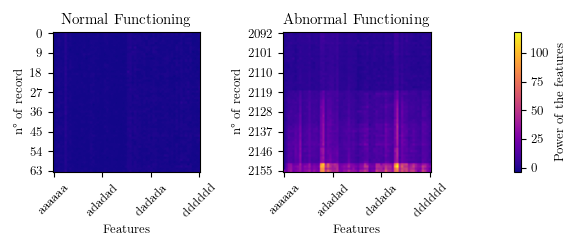
\includegraphics[scale=0.9]{images/Figure_5.png}
% \caption{Heatmap of the wavelet coefficients powers }
% \label{fig2}
% \end{figure}

% \begin{figure}[htbp]
%   \centering
%   \includesvg[width=\textwidth]{images/PMA_flowchart.svg}
% \caption{Predictive maintenance agent flowchart}
% \label{fig2}
% \end{figure}

% \begin{figure}[htbp]
%   \centering
%   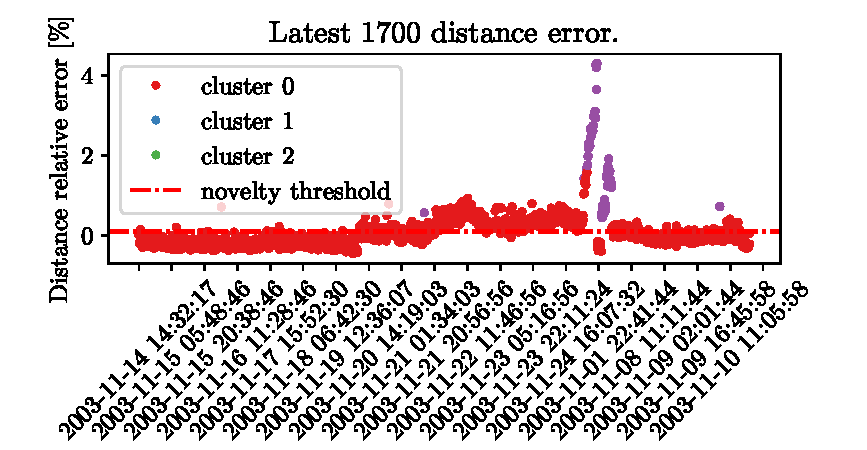
\includegraphics{images/Figure_1.pdf}
% \caption{Predictive maintenance agent flowchart}
% \label{fig2}
% \end{figure}